\documentclass[openright,twoside,11pt,a4paper]{scrartcl}  
\usepackage[T1]{fontenc}	%Tilde
\usepackage{courier}	%Tilde
\usepackage[ngerman]{babel}
%\usepackage{amsmath}
%\usepackage{amssymb}
%\usepackage[usenames]{color}	%Mehr Farben
%\usepackage{color}		%Farben
\usepackage{graphicx}	%Bilder
%\usepackage{cancel}	%zum Kürzen in Formeln
\usepackage{listings}	%Codehighlighting
\usepackage[utf8]{inputenc}	%Sonderzeichen nach utf8
\usepackage[dvipsname]{xcolor}	%Alle Farben
%\usepackage{tikz}	
%\usepackage{empheq}	%Formelboxen
%\usepackage{microtype}	
\renewcommand{\rmdefault}{phv} % Arial
\renewcommand{\sfdefault}{phv} % Arial
\usepackage[paper=a4paper,left=35mm,right=25mm,top=30mm,bottom=25mm]{geometry}



\begin{document}
	\lstset{classoffset=0,
		language=C++,
		basicstyle=\ttfamily,
		numbers=left,
		numberstyle=\tiny,
		inputencoding=utf8,
		emph={time, alarm, matrix_init, uint8_t, uint16_t},emphstyle=\color{blue},
		keywordstyle=\color{red},
		stringstyle=\color{red},
		commentstyle=\color{green},
		morecomment=[l][\color{magenta}]{\#},
		extendedchars=false,
		tabsize=2,
	}	


\begin{titlepage}
	\author{Moritz Nörenberg und Jacob Ueltzen}
	\title{Dokumentation zum Weckerprojekt}
	\date{}
	\maketitle
	\thispagestyle{empty}
\end{titlepage}
\newpage
\thispagestyle{empty}
\quad 
\newpage
\tableofcontents	\thispagestyle{empty}	\newpage	
\setcounter{page}{1}	
	
	\begin{flushleft}
		\section{Einführung}
		Im folgenden soll unser Weckerprojekt beschrieben werden, welches auf dem MSP-Education System umgesetzt werden sollte. Dabei sind folgende Vorgaben zu beachten gewesen:\\
		\begin{itemize}
			\item[1:] Weckuhr mit Anzeige von Uhrzeit, Datum, Wochentag und Alarmzeit über das LCD
			\item[2:] Eingabe und Justage von Uhrzeit, Alarmzeit und Datum
			\item[3:] Akustischer Weckalarm aus unterschiedlichen Tönen
			\item[4:] Nutzung der 4x4 LED Matrix zur Anzeige der Uhrzeit als Laufschrift (Stunden : Minuten)
		\end{itemize}
		Ich werde versuchen den Verlauf unserer Arbeit in dieser Dokumentation zu reproduzieren und die Funktionen und Module in der Reihenfolge zu erläutern, in welcher sie von uns implementiert wurden, um für den Betrachter verständlich zu machen, welchen Problemen wir bei unserer Arbeit begegnet sind und wie wir diese gelöst haben. Außerdem hoffe ich so eine bessere Verständlichkeit für unseren Quelltext vermitteln zu können. 
		\section{Uhrzeitanzeige}
		Begonnen haben wir zu aller erst damit, dass ir eine angezeigte Uhrzeit auf dem LCD des Education Systems angezeigt haben wollten. Dabei haben wir uns dafür entschieden folgendes struckt Element anzulegen:
		\begin{lstlisting}
			typedef struct
			{
			uint8_t sec;		//
			uint8_t min;
			uint8_t hour;
			uint8_t day;
			uint8_t mon;
			uint16_t year;
			} time_t;
			
			time_t time;
		\end{lstlisting}
		Dabei soll in den einzelnen Variablen jeweils der entsprechende Teil der Uhrzeit gespeichert werden. time.hour soll also nur den Wert der Stunde haben, um 21:10 Uhr also den Wert 21.\\
		Als nächstes brauchten wir eine Funktion, die uns die in time gespeicherten Werte auf dem LCD anzeigen kann. Für das ansteuern des LCD liegt im zur Vorlesung Mikrorechnerarchitekturen gehörigen Repository von Robert Fromm eine Header- und die zugehörige Source-Datei, die lcd.h und lcd.c, welche wir zu unserem Projekt hinzugefügt haben. Damit erhielten wir nun Zugriff auf sämtliche dort deklarierten und definierten Funktionen. Darunter auch die Funktion \lstinline[language=C++]|lcd_put_char()|, welche in der Lage ist einzelne  character auf dem LCD darzustellen. Da unser struckt time nun aber keine character Variablen speichert brauchten wir zusätzlich noch ein Funktion, welche die gespeicherte Zeit so umrechnet, dass sie mit der gegeben Funktion auf dem LCD ausgegeben werden kann. 
		\begin{lstlisting}
void outputtime()
{
lcd_put_char((time.hour - (time.hour % 10)) / 10 + 48);
lcd_put_char((time.hour % 10) + 48);
lcd_write(":");
lcd_put_char((time.min - (time.min % 10)) / 10 + 48);
lcd_put_char((time.min % 10) + 48);
lcd_write(":");
lcd_put_char((time.sec - (time.sec % 10)) / 10 + 48);
lcd_put_char((time.sec % 10) + 48);
}
		\end{lstlisting}
		Dabei berechnet die erste Zeile der Funktion den Zehner der Stunde und gibt diesen aus, die zweite Zeile berechnet den Einer der Stunde und gibt diesen aus und die Dritte Zeile gibt einen Doppelpunkt als Trennzeichen aus. Die 48 am Ende jeder Zeile sorgt dafür, dass auch die richtigen Zeichen ausgegeben werden. 48 ist in ASCII eine 0, also wird auf jeden errechneten wert diese 48 addiert um das entsprechende Zeichen zum Wert auszugeben. Auf die selbe Art wird noch mit Minuten und Sekunden verfahren.\\
		Ähnlich sind wir dann auch mit dem Datum verfahren, bis auf die Berechnung des Jahres, die mit dieser Methode recht umständlich und lang geworden wäre. Das Jahr haben wir daher in ein Array geschrieben, welches wir dann über die Funktion \lstinline[language=c++]|lcd_write()| ausgeben können, welche ebenfalls in der lcd.c definiert ist. \\
		\begin{lstlisting}
 	char Jahr[5];
	snprintf(Jahr, sizeof(Jahr), "%d", time.year);
	lcd_write(Jahr);
		\end{lstlisting}
		Damit ist nun die Ausgabe von Uhrzeit und Datum möglich, auch wenn sich diese noch nicht aktualisiert und nur über den Quellcode vordefinierte Werte annehmen kann. (Vgl. main.c line 29-34)
		
		\section{Aktualisierung der Uhrzeit}
		Für die sekündliche Aktualisierung der Uhrzeit war es nun nötig einen sekündlich auslösenden Interrupt zu bekommen. Dafür haben wir, wie in der Vorlesung gezeigt, den Watchdog-timer so initialisiert, dass er sekündlich einen Interrupt auslöst. 
		\begin{lstlisting}
	WDTCTL = WDTPW + WDTTMSEL + WDTCNTCL + WDTSSEL; 
	IE1 |= WDTIE; 
		\end{lstlisting}
		Bei auslösen dieses Interrupt Vektors wird unser Strukturelement time.sec um eins nach oben gezählt und außerdem für spätere Anwendungen auch das \lstinline[language=C++]|BIT0| in die Variable \lstinline[language=c++]|second_flag| geschrieben. Diese heißt nicht so, weil es in einer Form die zweite ist, sondern weil sie sekündlich auslöst.\newpage
		 \begin{lstlisting}
	 #pragma vector=WDT_VECTOR  
	 __interrupt
	 void WDT_ISR()  
	 {	//Interrupt Vektor: time.sec++
	 time.sec++;
	 second_flag = BIT0;
	 __low_power_mode_off_on_exit();
	 }
		 \end{lstlisting}
		 Damit kann nun die Sekundenanzeige im Sekundentakt nach oben zählen. Allerdings bisher nur ASCII Zeichen und selbst wenn man bei 0 anfangen lässt würde der Counter über die 10 hinaus zählen und die zugehörigen ASCII Zeichen auf dem LCD ausgeben. Dafür haben wir dann die Funktion \lstinline[language=c++]|time_correction| geschrieben. Hier nur ein Auszug daraus:
		 \begin{lstlisting}
	 void timeCorrection()    
	 {	//overflow handling aller Zeiteinheiten
	 if (time.sec > 59)
	 {
	 time.sec = 0;
	 time.min++;
	 
	 if (time.min > 59)
	 {
	 time.min = 0;
	 time.hour++;
	 ...
		 \end{lstlisting}
		 Diese Funktion geht in ähnlicher Form durch alles Elemente der Struktur time. Bei den Monaten ist es dann etwas komplizierter da die Monate unterschiedlich viele Tage haben können. Außerdem befindet sich in dieser Funktion auch noch die Berechnung der Schaltjahre:\newpage
		 \begin{lstlisting}
	...
	 else if (time.mon == 2)
	 {
		 if (time.year % 4 == 0 && time.year % 100 != 0
	 		|| time.year % 400 == 0)
	 	{
	 		if (time.day > 29)
	 		{
				 time.mon++;
				 time.day = 1;
	 		}
	 	}
	 	else
	 	{
	 		if (time.day > 28)
		 	{
				 time.mon++;
				 time.day = 1;
		 	}
	 	}
	 }
	 ...
		 \end{lstlisting}
		 Da es nun nur noch möglich ist existierende Daten und Uhrzeiten auszugeben und nicht Daten wie zum Beispiel den 30.Februar, der so nicht existieren kann, konnten wir uns nun as nächstes daran machen eine Berechnung für die Wochentage anzustellen. Dafür haben wir die von Gauß aufgestellte Formel zur Berechnung von Wochentagen zur Hilfe genommen, deren Gültigkeitsbereich zwischen dem 15.10.1582, dem Tag der Einführung des Gregorianischen Kalenders und dem Jahr 3000 liegt. \\Die Folgende Funktion berechnet die Lauf-variable \lstinline[language=c]!uint8_t weekdayi! , welche Werte zwischen 0 und 6 annehmen kann, die einen linearen Zusammenhang zum Wochentag haben. Ist \lstinline[language=c++]|weekdayi| gleich 0, so ist der errechnete Wochentag Sonntag, bei einer eins ein Montag usw. Die Ausgabe davon haben wir über eine switch-case Anweisung realisiert. Davon aber hier gleich nur einen Auszug.\newpage
		 \begin{lstlisting}
 void weekdayinit() 
 {//Berechnung von weekdayi mithilfe
 uint8_t h; //der Gauss'schen Wochentagsformel
 uint16_t k;
 
 if (time.mon <= 2)
 {
	 h = time.mon + 12;
	 k = time.year - 1;
 }
 else
 {
	 h = time.mon;
	 k = time.year;
 }
 
 weekdayi = (time.day + 2 * h + (3 * h + 3) / 5 + k + k / 4 - k / 100
 + k / 400 + 1) % 7;             //Wochentagsberechnung
 
 }
 
 
 void outputday() //Ausgabe des jeweiligen Wochentags
 {
	 lcd_gotoxy(0, 1);
	 switch (weekdayi)
	 {
	 case 0:
		 lcd_write("SUN,");
		 break;
	 case 1:
		 lcd_write("MON,");
		 break;
	 case 2:
		 lcd_write("TUE,");
		 break;
	 ...
}
		 \end{lstlisting}
		 Damit ist unser Wecker nun in der Lage zu einem Datum den richtigen Wochentag anzuzeigen und dabei die Zeit zu zählen. Wenn also die Zeit die richtige ist wäre der Wecker fertig. Das einzige, was nun also noch Fehlt, um die Zeitfunktionen des Weckers zu vollenden ist die Möglichkeit, Uhrzeit und Datum am Wecker selbst einstellen zu können.	\newpage	 
		 \section{Initialisierung des Weckers}
		 Wir haben zu beginn die einfachste Möglichkeit gewählt Uhrzeit und Datum des Weckers einzustellen, die uns einfiel. Diese beinhaltete jedoch keine Möglichkeit innerhalb des Einstellungsmenüs wieder einen Schritt zurück zu gehen. Hatte man zum Beispiel die Stunden bereits eingestellt und war weiter gegangen zu den Minuten, so gab es keine Möglichkeit wieder zu den Stunden zurückzukehren. Eigentlich haben wir dieses Problem zu einem anderen Zeitpunkt gelöst, da wir aber bei der Lösung diese Problems eine Menge Code verändert und gelöscht haben werde ich jetzt nur noch auf die letztendliche Lösung eingehen und einige Schritte in der Entstehung des Weckers auslassen.
		 \subsection{Einstellung der Uhrzeit}
	 	Für die Einstellung der Uhrzeit haben wir eine Funktion geschrieben, welche die momentan ausgegebene Uhrzeit verändern kann. Dafür wird eine Zählvariable eingeführt, die vom Drehencoder hoch oder runter gezählt werden kann. Also mussten wir zu aller erst den Drehencoder interruptfähig machen und eine hoch- und runterzähl Unterscheidung beifügen. Da wir das Grundprinzip für diese Funktionalität aber aus Robert Fromms GitHub Beispiel entnommen haben werde ich hier nicht tiefer darauf eingehen. Mithilfe des Drehencoder ist es uns nun aber möglich, dass wir über kurze if-schleifen eine Überlaufabfrage machen um keine unerlaubten Zahlen zu erreichen oder auch keine anderen ASCII Zeichen über das LCD Ausgegeben werden können. Hier ein Beispiel:
	 	\begin{lstlisting}
if (time.hour == 20)//Zehner der Stunden = 20
	{//Also noch max. 3 moeglich, da 24 nicht erlaubt ist
		if (a > 51)//51 in ASCII entsprich 3
		{
			a = 48;//48 entspricht 0
		}
		if (a < 48)
		{
			a = 51;
		}
	}
	else//Zehner der Stunden nicht 20
	{//Voller Zahlenumfang erlaubt
		if (a > 57)//entspricht 9
		{
			a = 48;
		}
		if (a < 48)
		{
			a = 57;
		}
	}
	 	\end{lstlisting}
	 	Dabei wird unsere Zählvariable a dauerhaft auf dem LCD ausgegeben, damit der Benutzer des Weckers auch sehen kann, was er einstellt. Ist der Nutzer Fertig mit dem einstellen eines Digits und drück den weiter oder zurück Button, dann wird der aktuelle Wert von \lstinline[language=c++]|a| als dezimal Ziffer umgerechnet im zugehörigen Struckt-Element gespeichert. Daraufhin wird \lstinline[language=c++]|a| wieder zu 0 gesetzt und der Cursor je nach Eingabe des Nutzers um eine Stelle nach vorn oder nach hinten verschoben.
	 	\begin{lstlisting}
if (button_flag & BIT0)           // Weiter-Button
{
	button_flag &= ~BIT0;
	time.hour = time.hour + (a - 48);
	a = 48;
	setupTimeState = setupTimeStateTenMin;
}
if (button_flag & BIT1)           // Zurueck-Button
{
	button_flag &= ~BIT1;
	time.hour = time.hour + (a - 48);
	a = 48;
	setupTimeState = setupTimeStateTenHour;
}
	 	\end{lstlisting}
	 	Dies ganze wird für jedes einzustellende Digit wiederholt und alles zusammen steht in einer switch-case Anweisung, die zwischen den verschiedenen Zuständen von \lstinline[language=c++]|setupTimeState| unterscheidet und somit die Navigation innerhalb des Menüs ermöglicht. \\
	 	\subsection{Einstellung des Datums}
	 	Bei der Einstellung des Datums sind wir auf die Selbe Weise Vorgegangen wie bisher bei der Uhrzeit. Da wir uns bei der Einstellung des Datums in einem anderen Menüpunkt befinden und dieser auch unabhängig von der Uhrzeiteinstellung sein soll haben wir dies alles in eine weiter Funktion geschrieben. Diese heißt \lstinline[language=c++,]|void setupdate()| und macht im Grunde das selbe wie die eben beschriebene Funktion, ist aber länger. Trotzdem werde ich hier nicht näher darauf eingehen, da dies nicht zu weiterem Verständnis der Funktionalität und dem Aufbau des Programmes beitragen würde.
	 	\subsection{(Neu)start des Weckers}
	 	Bei erstmaligen starten des Programms oder bei Neustart des Weckers, ob über den auf dem Education System verbauten Reset Button oder durch trennen der Stromverbindung, wird über eine Funktion Namens \lstinline[language=c++]|void startupscreen()|, die nur einmalig bei Neustart des Programms ausgeführt wird, die Initialisierung durchlaufen. Das bedeutet, dass der Benutzer auf dem LCD dazu aufgefordert wird die aktuelle Uhrzeit einzugeben und darauf hin die im Kapitel 4.1 beschriebene Funktion aufgerufen wird. Nachdem der Benutzer dann die Zeit eingegeben hat kann er durch bestätigen zur Einstellung des Datums kommen. Hierfür wird die im Kapitel 4.2 beschriebene Funktion aufgerufen. Wenn die Einstellung der Uhrzeit abgeschlossen ist und der Nutzer dies bestätigt wird noch die Funktion zur Wochentagsberechnung ausgeführt und auf dem LCD erscheinen dann die Worten $"$Initialisierung abgeschlossen$"$. Damit ist der Wecker vollständig initialisiert und wechselt automatisch in den Uhrzeit Bildschirm und beginnt damit die Uhrzeit zu zählen und anzuzeigen. \\
	 	Da die gerade beschriebene Funktion \lstinline[language=c++]|void startupscreen()|, nur aus aufrufen bereits bekannter Funktionen besteht werde ich hier kein Codebeispiel dazu zeigen. \\
	 	\section{Alarm}
	 	Da nun die Grundfunktionen eines Weckers gegeben sind war es an der Zeit sich um zusätzliche Funktionen zu kümmern. Der dabei von uns zuerst bearbeitete Punkt war die Weckfunktion. \\
	 	Da wir hier vieles Gleichzeitig und auch teilweise Dinge nicht so benutzt haben, wie wir sie uhrspr"unglich geschrieben haben werde ich für diesen Teil davon Abweichen den Code chronologisch zu erläutern, sondern hier die einzelnen Funktionalitäten der Weckfunktion erklären. Dadurch kann es dazu kommen, dass in einigen Beispielen Referenzen zu Funktionen stehen, die bisher noch nicht bekannt sind. Dies lässt sich leider nicht vermeiden und ich hoffe, dass das Verständnis unserer Vorgehensweise nicht darunter zu leiden hat.
	 	\subsection{Einstellen der Alarmzeit}
		 Für das einstellen der Weckzeit brauchten wir nun lediglich einen weiteren Menüpunkt und konnten dann wieder das Grundprinzip der vorangehend erläuterten Funktion zur Zeiteinstellung nutzen. Da diese Vorgehensweisen aber bereits bekannt sind werde ich nicht weiter darauf eingehen.\\
		 Zusätzlich haben wir uns auch ein weiteres struckt Element angelegt, welches wieder die Uhrzeitvariablen enthält und eine weitere Variable namens enable. Dieses Struckt kommt mit der Variable alarm und alarmold. Den Grund dafür werde ich später erläutern. \\
		 Da unser Vorgehen mit dem struct Element ähnlich dem vorherigen ist werde ich auch hier wieder nicht darauf eingehen.\\
	 	Weiterhin war es jedoch auch nötig dem Nutzer die Möglichkeit zu geben sich nicht wecken zu lassen. Dafür haben wir die Variable enable eingeführt, die grundsätzlich nur zwei Zustände haben kann. 1 zum einschalten des Weckers, was auf dem LCD als $"$EIN$"$ ausgegeben wird und 0, um die Weckfunktion auszuschalten, was auf dem Display des Weckers als $"$AUS$"$ angezeigt wird. Der Zustand von enable wird vom Nutzer auf die selbe Art eingestellt, wie die Einstellung der Weckzeit vorher. \\
	 	\ \\
	 	Um nun aber auch einen Weckvorgang zu bekommen brauchten wir noch etwas, dass die Aktuelle Zeit mit den in \lstinline[language=c++]|alarm| gespeicherten und vom Nutzer eingegebenen Werten vergleicht. Dafür haben wir folgende if-Anweisung so in unser Hauptprogramm geschrieben, dass sie dauerhaft wieder aufgerufen wird.
	 	\begin{lstlisting}
	 	 if (time.hour == alarm.hour && time.min == alarm.min
	 	&& alarm.sec == time.sec && alarm.enable == 1)
	 	{ 
	 		menuState = menuState_WAKEUP;
	 	}
	 	\end{lstlisting}
	 	Diese Schleife vergleicht alle einzelnen Elemente der Zeit mit denen, die im Alarm eingestellt worden sind. Dabei w"aren die Sekunden eigentlich gar nicht von n"oten gewesen, da die Weckzeit nur auf volle Minuten gestellt werden kann. Dennoch vergleichen wir diese mit, da wir somit das Problem umgehen k"onnen, dass der Wecker eine ganze Minute lang durch klingeln w"urde, ohne das der Nutzer in der Lage w"are das Wecken zu unterbrechen. Der Wert von \lstinline[language=c++]|alarm.sec| kann nicht vom Nutzer ge"andert werden und ist 0 by default. Somit l"ost der Alarm nur zur vollen Minute der eingestellten Weckzeit aus und der Kopf der if-Schleife ist auch nur diese eine Sekunde lang wahr. W"urde der Nutzer versuchen innerhalb dieser Sekunde den Alarm wieder abzustellen k"onnte es zu Fehlern kommen und der Abstellknopf m"usste ein weiteres Mal gedr"uckt werden.\\
	 	Die Zuweisung im Rumpf der Schleife versetzt den Counter unseres Menü-Zählers in Alarmzustand. Das bedeutet, dass sich unsere große switch-case Anweisung in den Zustand \lstinline[language=c++]|WAKEUP| begibt. Dieser wird im Folgenden Kapitel erläutert.
	 	\subsection{Abstellen des Alarms}
	 	Zum Abstellen des Alarms bedarf es eines einzelnen Knopfdruckes. Durch unsere switch-case Anweisung können wir dies ganz einfach dadurch realisieren, dass wir die Abbruchbedingung in den Kopf einer If-Schleife schreiben und in deren Rumpf wiederum den neuen Zustand für den Menü-Counter definieren. Dies ist zu sehen in den Zeilen 10 bis 12 des folgenden Beispiels:
	 	\begin{lstlisting}
	 	 
	 	 case menuState_WAKEUP:
	 	 lcd_clear();
	 	 matrix_clear();
	 	 setalarmtone();
	 	 lcd_gotoxy(4, 0);
	 	 lcd_write("ALARM!");
	 	 timeCorrection();
	 	 
	 	 if (button_flag & BIT0)
	 	 {
		 	 menuState = menuState_TIME;
		 	 stopalarmtone();
		 	 lcd_clear();
		 	 button_flag &= ~BIT0;
	 	 }
	 	 
	 	\end{lstlisting}
	 	Dabei wird im Rumpf der Schleife zusätzlich noch in Zeile 13 der Alarmton ausgeschaltet, der in Zeile 5 aktiviert wurde und das LCD gelöscht, da es während des Weckens mit dem Wort $"$ALARM$"$ beschrieben wird, wie in Zeile 7 zu sehen ist. Dazu jedoch später noch mehr. Außerdem wird auch hier wieder das \lstinline[]|BIT0| getoggelt um erneutes Auslösen ohne ein weiteres Drücken des Tasters zu verhindern.\\
	 	Die Funktion \lstinline[language=c==++]|timeCorrection()| muss mit während des Weckvorgangs ausgef"uhrt werde, da der Wecker selbst sonst im Hintergrund nicht weiter z"ahlen w"urde. \\
	 
	 	\subsection{Klingeln des Weckers}
	 	Um den Wecker klingeln zu lassen muss der Nutzer also eine valide Alarmzeit eingegeben haben und das alarm.enable bit auf eins gesetzt haben. Wenn dies geschehen ist, ist auch auf dem Hauptbildschirm ein $"$A$"$ zu sehen, welches den Nutzer darauf hin weißt, dass ein Alarm aktiv ist. \\
	 	\ \\
	 	Die Tonausgabe wurde mittels des CCR2 Registers und Timer A realisiert. Hierfür konfigurierten wir Timer A so, dass die Auxillary clock von Timer A verwendet wird. Außerdem haben wir uns für den kontinuierlichen Modus des Hochzählens entschieden. Verscheidene Töne haben wir mit verschiedenen Einträgen in das CCR2 Register realisiert. Diese werden durch die Variable toneccr in das CCR2 Register geschrieben. Zunächst bei der Initialisierung vor der while-Schleife im Hauptprogramm, danach wird viertelsekündlich ein anderer Wert in das CCR2 Register eingetragen. Das geschieht in der Interruptservicesoutine für den Watchdogtimer. Abhängig von der dort hochzählenden clock-Variable wird einer von vier verschiedenen Werten in das CCR2 Register geschrieben. Die Werte im CCR2 Register bestimmen, nach wie vielen Auxillary Taktzyklen der Lautsprecherausgang getoggelt werden soll. Somit werden Rechtecksignale verschiedener Frequenz erzeugt.
	 	\begin{lstlisting}
	 	 case 4:	// CCR2 Interrupt
	 		CCR2 += toneccr;
		 	if (clock == 0)
		 	{
		 		toneccr = 30;
		 	}
		 	else if (clock == 1)
		 	{
		 		toneccr = 37;
		 	}
		 	else if (clock == 2)
		 	{
		 		toneccr = 52;
		 	}
		 	else if (clock == 3)
		 	{
		 		toneccr = 74;
		 	}
	 		break;
	 	\end{lstlisting}

	 	
	 	\section{Die LED-Matrix}
	 	Ein weiteres Feature zum Wecker, welches laut den Vorgaben programmiert werden muss ist die LED-Matrix. Zum Ansteuern der Matrix haben wir uns die von Robert Fromm geschrieben \lstinline[language=c++]|matrix.c| und die dazugehörige \lstinline[language=c++]|matrix.h| in unser Projekt eingebunden. Dort sind unter anderem Funktionen wie die \lstinline[language=c++]|matrix_init()|, welche zur Benutzung der LED-Matrix zwangsläufig von Nöten ist. Auch einige andere essentielle Funktionen sind in diesen Dateien definiert, die in unserem Projekt Verwendung finden. Diese werde ich jedoch nicht alle einzeln erläutern.\\
	 	\ \\
	 	Zu Beginn haben wir eine Funktion geschrieben, welche die komplette Matrix zum leuchten bringen kann und eine, welche alle LED's der Matrix wieder ausschaltet. Benutzt haben wir davon letztendlich nur die zum ausschalten, aber behalten haben wir die andere für Verwendung zu späteren Zeitpunkten trotzdem. Im Beispiel ist nun die Verwendete Funktion zum ausschalten der Matrix zu sehen:
	 	\begin{lstlisting}
	 	void matrix_clear()
	 	{
		 	matrix_write_row(0, 0b0000);
		 	matrix_write_row(1, 0b0000);
		 	matrix_write_row(2, 0b0000);
		 	matrix_write_row(3, 0b0000);
	 	}
	 	\end{lstlisting}
	 	Diese Funktion wurde bereits im Kapitel 5.2 im Codebeispiel zum Alarm benutzt. Sie tut nichts weiter, als dass sie alle Elemente der Matrix mit Nullen beschreibt, also alle LED's ausschaltet.\\
	 	Die Funktion zum einschalten der Matrix sieht dieser sehr ähnlich, bis auf dass in den Klammern als zweiter wert überall eine binäre 15, also vier Einsen stehen um die einzelnen LED's der Matrix einzuschalten. \\
	 	\ \\
	 	Für das Lauflicht auf der Matrix ist es wichtig, dass die einzelnen anzuzeigenden Zeichen irgendwo hinterlegt sind. Da wir nur die Zeit anzeigen wollen brauchten wir die Zahlen von 0 bis 9. Wie diese auf der Matrix aussehen sollen ist im folgenden Vektor hinterlegt.
	 	\begin{lstlisting}
	 	uint8_t zahlen[10][3] = {
	 			{ 0b1111, 0b1001, 0b1111 },    //0
			 	{ 0b1010, 0b1111, 0b1000 },    //1
			 	{ 0b1001, 0b1101, 0b1011 },    //2
			 	{ 0b1001, 0b1011, 0b1111 },    //3
			 	{ 0b0111, 0b0100, 0b1110 },    //4
			 	{ 0b1011, 0b1011, 0b1101 },    //5
			 	{ 0b1111, 0b1011, 0b1101 },    //6
			 	{ 0b0001, 0b0101, 0b1111 },    //7
			 	{ 0b1111, 0b1011, 0b1111 },    //8
			 	{ 0b1011, 0b1011, 0b1111 }    //9
	 	};
	 	\end{lstlisting}
	 	Dabei bilden immer drei der Zeilen eine Zahl. Jede der Zeilen steht dabei für eine Spalte auf der Matrix. Bildlich vorstellen kann man sich das am besten am Beispiel der Null. Da hat der erste Eintrag vier Einsen, in der ersten Spalte der Matrix sind also alle LED's an. Der zweite Eintrag besteht aus zwei Nullen umgeben von je einer Eins, daraus resultiert in der zweiten Spalte der Matrix, dass die obere und die untere LED an sind, die dazwischen aus. Der dritte Eintrag ist wieder gleich dem ersten, es entsteht wieder eine voll eingeschaltete Spalte. Das hintereinander ergibt das ungefähre Abbild einer Null in den ersten drei Spalten der Matrix. \\
	 	Damit sind wir nun in der Lage eine Zahl zur Zeit in der Matrix anzuzeigen, jedoch haben wir noch nicht das geforderte Lauflicht. Dafür haben wir uns eine Vektor mit 20 Einträgen definiert, der in einer Funktion immer mit der momentanen Zeit und denn nötigen Trenn- und Leerzeichen beschrieben wird. Dies sieht wie folgt aus:
	 	\begin{lstlisting}
void array_input()
{	...
	output[3] = 0b0000;
	output[4] = zahlen[(time.hour - (time.hour % 10)) / 10][0];
	output[5] = zahlen[(time.hour - (time.hour % 10)) / 10][1];
	output[6] = zahlen[(time.hour - (time.hour % 10)) / 10][2];
	output[7] = 0b0000;
	output[8] = zahlen[time.hour % 10][0];
	output[9] = zahlen[time.hour % 10][1];
	output[10] = zahlen[time.hour % 10][2];
	output[11] = 0b0000;
	output[12] = 0b1010;
	...
}
	 	\end{lstlisting}
	 	output[] ist der bereits genannte Vektor. Seine ersten vier Elemente werden nur mit Nullen beschrieben, damit die Uhrzeit "reinlaufen" kann und nicht bei Aufruf der Funktion bereits die erste Zahl auf der Matrix steht. Davon ist hier jedoch nur noch das vierte Element zu sehen. \\
	 	Die Zeilen 4 bis 6 des Codebeispiels errechnen die Zehner der Stunde und verlangen den Wert des Vektors Zahlen in Abhängigkeit der errechneten Stunde. Das zweite Argument des Vektors zahlen ist dabei für die drei benötigten Spalten verantwortlich, die benötigt werden, um eine Zahl darzustellen.\\
	 	In Zeile 7 ist dann eine Leerzeile als Trennung zwischen den Zahlen eingefügt, dann wiederholt sich das ganze mit den Einern der Stunde und in Zeile 12 ist ein Doppelpunkt als Trennung zwischen Stunden und Minuten eingefügt. Danach wiederholt sich das ganze noch für die Minuten, was hier jetzt aber nicht mit abgebildet ist, da das Vorgehen dafür identisch ist.\\
	 	\ \\
	 	Für das Lauflicht ist nun die Grundlage gelegt. Ein Vektor, der die gesamte Uhrzeit so enthält, inklusive der Trenn- und Leerzeichen, die benötigt werden um die Zeit lesen zu können. Da die Matrix aber nur vier Elemente breit ist und wir 20 haben kommt nun das laufen ins Spiel. Dafür haben wir eine weitere Funktion geschrieben, die dafür sogt, dass immer nur vier Elemente unseres Vektors \lstinline[]|output[]| auf der Matrix ausgibt:
	 	\begin{lstlisting}
void array_output()
{
	if (k > 20)
	{
		k = 0;
	}
	array_input();
	matrix_write_row(3, output[k + 3]);
	matrix_write_row(2, output[k + 2]);
	matrix_write_row(1, output[k + 1]);
	matrix_write_row(0, output[k]);
	k++;
}
	 	\end{lstlisting}
	 	Dabei werden alle vier Spalten der Matrix beschrieben und zwar mit den Werten, die im vorher beschriebenen Vektor stehen und das in Abhängigkeit der Variablen k. Diese ist eine lokale variable, die bei jedem Funktionsaufruf um eins nach oben gezählt wird und bei 21 auf 0 zurück gesetzt wird, damit nicht irgendwelche Elemente des Vektors \lstinline[]|output[]| angefordert werden, die es gar nicht gibt. Nun wird in die Spalte ganz links auf der Matrix der Wert des Vektors \lstinline[]|output[k]| geschrieben und in die nächste Spalte  der Wert von k+1 usw. So sind weiterhin die zusammengehörigen Zahlen zu sehen und da k bei jedem Durchlauf um eins erhöht wird bewegt sich die Schrift mit der Zeit nach links.\\
	 	Aufgerufen wird die Funktion im Hauptprogramm. Da wir die Matrix schneller laufen lassen wollten als nur mit einer Spalte pro Sekunde haben wir hierfür den Interrupt Vektor des Watchdog-Timers so verändert, dass er zwei Flags ausgibt, die \lstinline[]|clock_flag| und die bereits erwähnte \lstinline[]|second_flag|. \newpage
	 	\begin{lstlisting}
#pragma vector=WDT_VECTOR    
void WDT_ISR()
{	//interrupt vektor fuer time++ sekuendlich und clock++ viertelsekuendlich
	clock++;
	clock_flag |= BIT0;
	if (clock > 3)
	{
		clock = 0;
		time.sec++;
		second_flag = BIT0;
	}
	__low_power_mode_off_on_exit();
}
	 	\end{lstlisting}
	 	Der Aufruf der Funktion sieht dann folgendermaßen aus:
	 	\begin{lstlisting}
 if (clock_flag & BIT0)
{
	clock_flag &= ~BIT0;
	array_output();
}
	 	\end{lstlisting}
	 	Damit ist unser Wecker mit all seinen Benötigten und zusätzlichen Funktionen fertig. Er kann die Uhrzeit über das LCD anzeigen, sie lässt sich auch einstellen, es gibt eine Weckfunktion und die LED-Matrix Zeigt immer die Aktuelle Zeit an.\\
	 	\ \\
	 	Daraus ergibt sich der folgende Programm-Ablaufplan:
	 	\begin{figure}[htbp] 
	 		\centering
	 		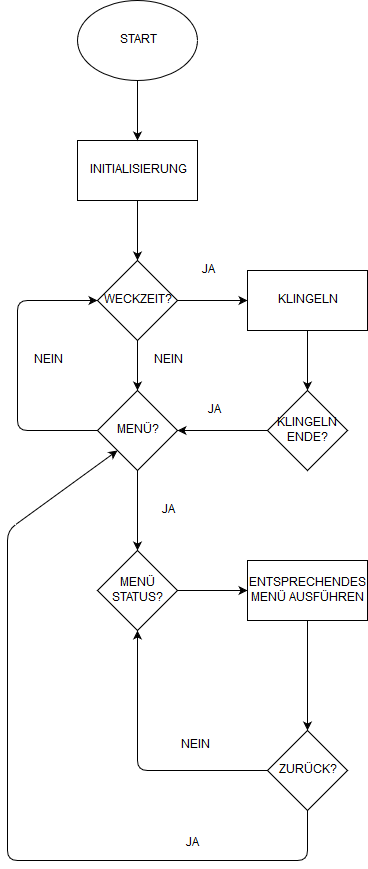
\includegraphics[width=0.6\textwidth]{Untitled Diagram.png}
	 		%\caption{}
	 		\label{fig:Bild1}
	 	\end{figure}

	\end{flushleft}
\end{document}